\documentclass[10pt]{article}
\usepackage[polish]{babel}
\usepackage[utf8]{inputenc}
\usepackage[T1]{fontenc}
\usepackage{amsmath}
\usepackage{amsfonts}
\usepackage{amssymb}
\usepackage[version=4]{mhchem}
\usepackage{stmaryrd}
\usepackage{graphicx}
\usepackage[export]{adjustbox}
\graphicspath{ {./images/} }

\title{LIGA MATEMATYCZNA \\
 im. Zdzisława Matuskiego \\
 GRUDZIEŃ 2014 \\
 SZKOŁA PODSTAWOWA }

\author{}
\date{}


\begin{document}
\maketitle
\section*{ZADANIE 1.}
Mikołaj przydzielał siedmiu elfom prezenty do rozdania. Kolejno każdy otrzymywał po jednej paczce. Kiedy każdy elf miał już 18 prezentów pozostała reszta, która nie wystarczyła, by każdy otrzymał jeszcze po jednym. Reszte oddali Mikołajowi. Ile prezentów było do rozdania?

\section*{ZADANIE 2.}
Na kiermaszu przedświątecznym zaplanowano sprzedaż 400 bombek choinkowych po 16 zł za sztukę. Po sprzedaniu \(30 \%\) bombek okazało się, że część popękała w czasie transportu. Odłożono więc te bombki. Aby uzyskać zaplanowany przychód, pozostałe bombki zostały sprzedane po \(20 \mathrm{zł}\) za sztukę. Ile bombek popękało podczas transportu?

\section*{ZADANIE 3.}
Używając tylko cyfr 2 i 8 (być może kilkukrotnie) zapisz najmniejszą liczbę naturalną podzielną przez 9 oraz najmniejszą liczbę naturalną podzielną przez 12.

\section*{ZADANIE 4.}
Rozetnij kwadrat na cztery jednakowe części tak, aby w każdej znalazły się trzy kółka.\\
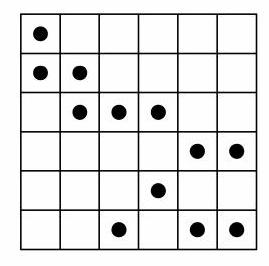
\includegraphics[max width=\textwidth, center]{2024_11_21_428684ae64167c130f83g-1(1)}

\section*{ZADANIE 5.}
Z trzech trójkątów prostokątnych równoramiennych zbudowano choinke, jak na rysunku. Podstawa największego trójkąta ma długość 20 cm . Podstawa następnego jest umieszczona w połowie wysokości poprzedniego trójkąta. Każdy kolejny trójkąt jest o 2 cm niższy. Oblicz pole powierzchni największego i najmniejszego trójkąta.\\
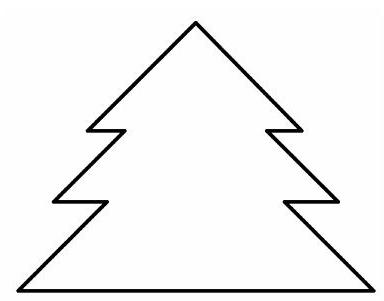
\includegraphics[max width=\textwidth, center]{2024_11_21_428684ae64167c130f83g-1}


\end{document}